%%%%%%%%%%%%%%%%%%%%%%%%%%%%%%%%%%%%%%%%%%%%%%%%%%%%%%%%%%%
% EPFL report package, main thesis file Goal: provide formatting for theses and
% project reports Template's Author: Mathias Payer <mathias.payer@epfl.ch>
% Thesis's Author : Arnaud Pannatier <arnaud.pannatier@epfl.ch>
%%%%%%%%%%%%%%%%%%%%%%%%%%%%%%%%%%%%%%%%%%%%%%%%%%%%%%%%%%%
\documentclass[a4paper,11pt,oneside]{report}
% Options: MScThesis, BScThesis, MScProject, BScProject
\usepackage[MScThesis]{EPFLreport} \usepackage{xspace}

\title{A Control Plane in Time and Space for Locality-Preserving Blockchains}
\author{Arnaud Pannatier} \supervisor{Cristina Basescu} \adviser{Prof. Bryan
Ford}
%\coadviser{Second Adviser}
\expert{\color{red}The External Reviewer\color{black}}

\newcommand{\sysname}{FooSystem\xspace}

\begin{document}

\maketitle 

\maketoc


%%%%%%%%%%%%%%%%%%%%
\chapter{Background}
%%%%%%%%%%%%%%%%%%%%

%%%% Plan
% - Crux (??)
% - Nyle (7-8p) - General description - What is already implemented - Next
%   steps
% (motivation for the control plane)
%%%%%%%%%%%%%%%%%%

This Master Thesis is part of a biggest structure that concerns
locality-preserving systems. In particular, it builds upon two different
systems CRUX\cite{basescu2014crux} and is part of Nyle.This section describes
the two different projects. 

\section{CRUX}

%%%% General Presentation
% - Solution to partition
% - General idea
% - Small Overhead
% - Generality 
% - CAP Theorem
%%%%%%%%%%%%%%%%%%
\subsection{General Presentation} CRUX introduces a smart way of dealing with
partitions in decentralized systems. The purpose is the following : partitions
occur in decentralized system. But one can maybe try to find a solution to
reduce their effects on the global system. For example, if a partition occurs,
there is no reason that nodes that are functioning in the same side of the
partition should stop working because of the partition. 

The general idea is that a system can be replicated at different scales, from
very local to global.  With the additional property than each replicated system
will continue to work correctly if no partition splits it. If a global
partition occur, then the global region might not work, but all the replicated
system in local regions will still work. Which is solving the mentioned problem
: nodes working on the same of the partition will continue to work.

This solution comes with an overhead, as the system should be replicated in all
the regions. But there are some ways of reducing this overhead, in a way that
it stays reasonable and that the resistance to partition is maintained. To
reduce this overhead, CRUX algorithm for regions creation presented below
ensure that the proper number of regions is created, in a manner that the
overhead stays reasonable and that the partition resistance stays efficient. If
CRUX is used for a particular, known system, overhead can be even more reduced.
As the systems are replicated in every region, most of the data is replicated
along the regions. So one might actually deep inside the specification of one
system and manages not to store twice the same data. But this overpass a bit
the goal of CRUX, which wants to be the more general possible. 

Indeed, the principal force of CRUX is that it is applicable to any distributed
system, as no particular hypothesis on the system is made. It only starts from
one simple idea : one system can be replicated at smaller scale to ensure
partition resistance. 

% TODO : do more research on that.
A note should be made about the CAP-theorem. Recall that this theorem states
that no system can be consistent, available and partition-resistant at the same
time. It seems that this solution is adding partition tolerance to available
and consistent system. Thus leading to the violation of the theorem. But it is
not exactly the case, as the created system only ensure that nodes can still
work in the same side of a partition. But the region split by the partition is
not working anymore. Even if the system can still work on the same side of a
partition, it's not partition resistant.

%%%% Common Tools
% - Approximation distance oracle
% - Bunch
% - Cluster
% - ARA 
%%%%%%%%%%%%%%%%%%
\subsection{Common Tools :  ARAs} This section describes how to create the
regions that are used to replicate the system. These regions are used by Nyle
as well therefore we will describe it in detail. 

These regions are called \textit{Available Responsive Areas}, in each region a
copy of the replicated system is deployed. 

To create these regions each node will participate first at a lottery. Each
node starts at level 0. Then each node go to the next level with probability
$p$. This procedure repeats at each level, and stop when no nodes are promoted
to the next level. This first empty level is called $k$. 

\begin{table}[] \begin{tabular}{rrrrr} & 100 & 200 & 500 & 1000 \\ \hline
\multicolumn{1}{r|}{0} & 90  & 180 & 450 & 900  \\ \multicolumn{1}{r|}{1} & 9
& 18  & 45  & 90   \\ \multicolumn{1}{r|}{2} & 1   & 2   & 5   & 9 \\
\multicolumn{1}{r|}{3} & 0   & 0   & 0   & 1   \end{tabular} \caption{Example
of lottery with $P = 0.1$ where $k= 3$ for $N= 100,200,500$ and $4$ for $N =
1000$} \end{table}

Then each node can compute two quantities that will be necessary to create
\textit{ARAs}. Their bunch and their cluster. 

\paragraph{Bunch} A node can compute its bunch in the following manner. It
looks at every other nodes by order of distances in ascending order and
includes it in its bunch if its level is not smaller than the one it encounters
so far, including its own level. 
% TODO include image of Bunch


\paragraph{Cluster} A cluster is a complementary concept. The cluster of node
$A$ is defined as the set of other nodes that have $A$ in their bunch. 
% TODO include image of Cluster.

The smallest region radius $R_{min}$ is defined for the whole system. Each node
will construct ARA's around itself starting at $R_{min}$ and doubling the
radius at each time. It stops at the first ARA's that is covering its entire
cluster. 

By the lottery, most nodes will be level-zero nodes. Therefore their cluster
supposed to be small, conducting to the creation of a small number of ARA's.
The small number of nodes that are at level $k-1$ will have every other nodes
in their cluster by construction. This means that there will be at least one
ARA that covers the whole system. 

%%%% Nyle
%  - Problems it solves - Link with CRUX - Environment - Type of Blockchain 
% - What is already implemented 
% - Next steps. 
%%%%%%%%%%%%%%%%%%%%%%%%%%%%%
\section{Nyle}

Nyle is cryptocurrency, that uses locality to answer some classical problems of
a blockchain systems. Two main problems are addressed: WW3 scenarios and
approval time for a transaction.
 
 \paragraph{WW3 Scenarios} \label{WW3} In case of a WW3, we can expect to have
 at least a long-lasting partition that will split the system in two. This is a
 problem for classical cryptocurrencies, because for a block to be approved,
 the users are supposed to wait to have a global consensus. This consensus will
 not be reached with a long-lasting partition and therefore it will create
 problems for classical cryptocurrencies. Nyle solve this issue by design using
 locality.

\paragraph{Approval Time for a Transaction} \label{approve_time} Another issue
with waiting global consensus is that it usually takes a long time. If we want
to use a cryptocurrency in a daily life, we want to solve that problem to be
able to validate (at least partially) a transaction relatively fast. The
solution provided by Nyle use locality again: with Nyle a transaction is
validated at different levels, and it is up to the user to wait a local, or
global validation for a transaction.

\subsection{Locality : From CRUX to Nyle}

In order to have the locality properties, Nyle uses a similar design than CRUX
but applies it in the specific case of a cryptocurrency. It assumes the same
Network model as in CRUX (set of nodes that are connected through an
Internet-like network,...). It uses the landmark technique from
approximate-distance oracles and creates ARAs, with the same strategies. So it
will provide the same properties for the network (and bunches, clusters,...)
and the ARAs.

So the ARA is the representation of the region. In each of these regions there
will be a copy of the same system, in the case of Nyle the system is a
blockchain. So each region will have its own blockchain and validate all the
transactions between the nodes that are included in it. Some nodes can be
included in different regions, and they will send their transactions to all the
regions they are part of. Which ensure that each blockchain will be updated
each time there is a transaction that concerns one of its nodes.

\subsection{Stable environment vs Byzantine evolving system}

The big difference between CRUX and NYLE is that the purpose of CRUX is to work
in environments where machines are relatively "stable" which means that they
are not supposed to churn or to crash often, and more, where the machines are
not supposed to move. This is not the case for Nyle : if we have a
cryptocurrency, we can expect to have malicious, deficient and/or moving users.
This will add some difficulties that will be managed by the protocol.

\subsection{Blockchain System} \label{blockchain_subsection}

Each region will have its own blockchain, in Nyle the choice for the blockchain
will be chosen between Omniledger or ByzCoin. But it can be generalized to any
kind of blockchain.

\subsection{What is already implemented for Nyle} \subsubsection{Transaction
validation} We already have a protocol that validates a transaction.

\subsubsection{Block storage on node} As each node will participate in
different regions (from very local to world-wide), it will need to store the
blockchains for all of these region. We have a method that reduces the
redundancy, by only storing the hash of a block instead of the full block at
each level. 

\subsubsection{Proof-of-Location} We already have a protocol for controlling
the distance from a new node to the rest of the nodes. And that assures no one
cheats by giving false distances. 


\subsection{Next Steps} Here is the structure of Nyle :

\begin{itemize} 
\item Based on the proof-of-location, build a CRUX-like network
\item In each of the region of the regions build a Blockchain 
(see \ref{blockchain_subsection})
\item Use the transaction validation to  give info on the validated region
(see \ref{approve_time} (Approval time for a transaction))
\item Dealing with moving actors.
\item Dealing with double-spending issues
(if a node spend the same coin in different regions) 
(see \ref{WW3} WW3 Scenarios) 
\item (Investigate if this design is open to other errors)
\end{itemize}

%%%%% TODO : add general description 
%%%%% Motivation
% - Already have a system working for non-byzantine no-churn system 
% - Dealing with these problems can be done by dealing nodes insertion,
            %   deletion and moving.
% - If we solve that then we can return to the previous system and everything
            %   should be working
%%%%%%%%%%%%%%%
\subsection{Purpose of this project : motivation for a control plane} CRUX
propose a system that is working in stable system (with low-churn) and where
nodes does not move too much. As this situation corresponds to some systems
like wide-area database, ... It is definitely not the case of a crypto-money.
For these kind of system, one can expect to have at least some churn, some
moving nodes and some adversarial nodes.  If the system have a precise protocol
for dealing with nodes entering, leaving and moving in the system, then the
problem of the evolution of the system is solved. Indeed the churn phenomenon
can be describes as some nodes leaving the system and optionally reentering
later. 

Therefore the purpose of the control plane will be to deal with the evolution
of the regions that follows the evolution of the nodes in the system. Once that
problem is solved, the blockchain can be replicated in the evolving region and
the strategy will be the same as in CRUX. 

Thus this project introduce a control plane, that is in charge of the evolution
of the nodes in the system. In particular, it will be in charge of dealing with
the nodes joining, leaving and moving in the global system. If the blockchains
is replicated in all the regions, the control plane will be global. 

%%%%%%%%%%%%%%%%
\chapter{Control Plane : Design}
%%%%%%%%%%%%%%%%


%%%%%%%%% 
%  - Problem definition (Hypothesis, Goals, ...) (2-3p) 
%%  - Hypothesis on the threat model
%  - First version: Simple Control Plane (15-20p ?) 
%%  - Graphs: Control flow, Protocol flow trough time 
%%  - Tools: Description of each subprotocols 
% %%%(consensus via Blscosi, gossips protocols, ...). 
%%   - Discussion
%%%%  - Advantages, prove that it fulfils the goal
%%%%%%  - Graph of difference between system without control plane and with. 
%%%%  - Drawback (evaluation of computational, memory and communication costs)
%%%%%%  - With graphs
%%  - Security  Analysis 
%%%%% - 2-3 scenarios illustrating malicious behaviors (written and/or with implementation)
%%%%%%%%%%%%%%%%%%%%%%%%%%%%%%%%%%%%%%%%%%%%%%%
This part will describe the design of the Control Plane, which has the mission
to solve the problem of node insertion, deletion and movement inside the
system. Allowing to use a CRUX-like region creation algorithm in an environment
with churn. 

\section{Problem definition}
%%%%%%%%%%%%%% Problem definition
%% Hypothesis : 
%%   - one-to-one communication
%%   - synchrone network
%%   - Correlation between pings and distances
%%   - Nodes are malicious
%%   - Adversary can delay communication
%%%%%%%%%%%%%%%%%%%%%%%%

\subsection{Hypothesis} Three hypotheses are made on the network. First it
assumes an internet-like network with one-to-one communication. Each node is
able to contact any other nodes. The network is supposed to be synchrone. This
means that every message sent by a node to another will arrive in order, and
that a message that is sent will be received within a given window of time. The
third hypothesis is made on the geometry of the network. It states that for
small pings (under 100ms) the ping time is actually correlated with the
distance between two nodes. This is a result from \cite{locality-result} on
which we build the locality properties of the system. 

\subsection{Threat model}
%% Todo : when adversarial model is done, depending on results. 



%%%% mostly copied from https://docs.google.com/document/d/1xz1jTphKqxxkAucdh_oOqsFXH147Cjlzcnjmt-yx-f8/edit#heading=h.aq4k1vxbt0t0
\section{General Presentation}

The Control Plane is composed of five different components [FIG. \ref{fig:modules}], each
necessary to solves different part of the problem. It needs a membership
component, to define precisely which nodes are in the system at any time. It
needs a locality component which gives the distance between two nodes in the
system. Then it needs a region management component, which will draw the
regions based on the membership and the locality. The time will be split into
epochs, a component is in charge of dealing that aspect. And finally, the
control plane is in charge of answering some requests linked to the location
and presence of the nodes in the system. Each will be described in detail
below. 


\begin{figure}[!h] \centering
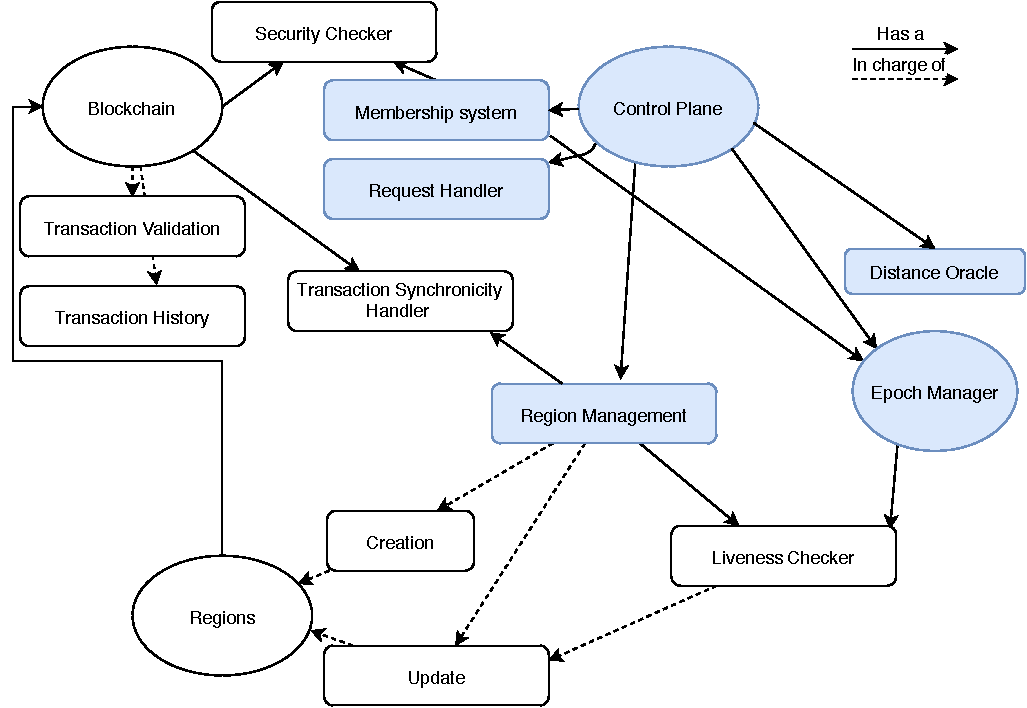
\includegraphics[width=400pt]{figures/Nyle_components} \caption{List of modules
of Nyle} \label{fig:modules} \end{figure}


\subsection{Membership Component}

At each epoch, a registry contract containing a summary of all participants is
created. Registration use endorsement (for example solution to a proof-of-work
problem).  This system will be global. Nodes can ask the participants of the
system to know the identity of other nodes. To validate a new contract  it
should be signed by the majority of the nodes of the previous epochs.

\subsection{Locality Component}

 The role of the locality component is to give all pairwise latencies between
 nodes of the system. We assume it already exists (distance oracle), or it can
 be computed by nodes. In the first model all pairwise latencies is computed
 between each node and every node agree on them via consensus. 
 
 \subsection{Region Component} This component is used to create and update
 regions. For the simple case, this part will be based on CRUX. At each epoch
 CRUX is run based on the new registration, and regions are created.
 
 \subsection{Epoch Component} The epoch manager is linked to the membership
 system (we allow to change membership at the beginning of one epoch). New
 nodes can join at the beginning of one epoch. If nodes have moved, the region
 component will change or maintain their assignment at the beginning of one
 epoch. 

Epochs happen at a defined rhythm (e.g. one day). This frequency can be
shortened to ensure that nodes that want to join do not wait too long, or made
longer if one wants regions not to be redrawn too frequently. 

\subsection{Request Handler} The control plane is the right part to get
requests as it is aware of the nodes location and region assignment. It will be
in charge of answering the request for nodes assignment and nodes location. 

\begin{figure}[!h] \centering
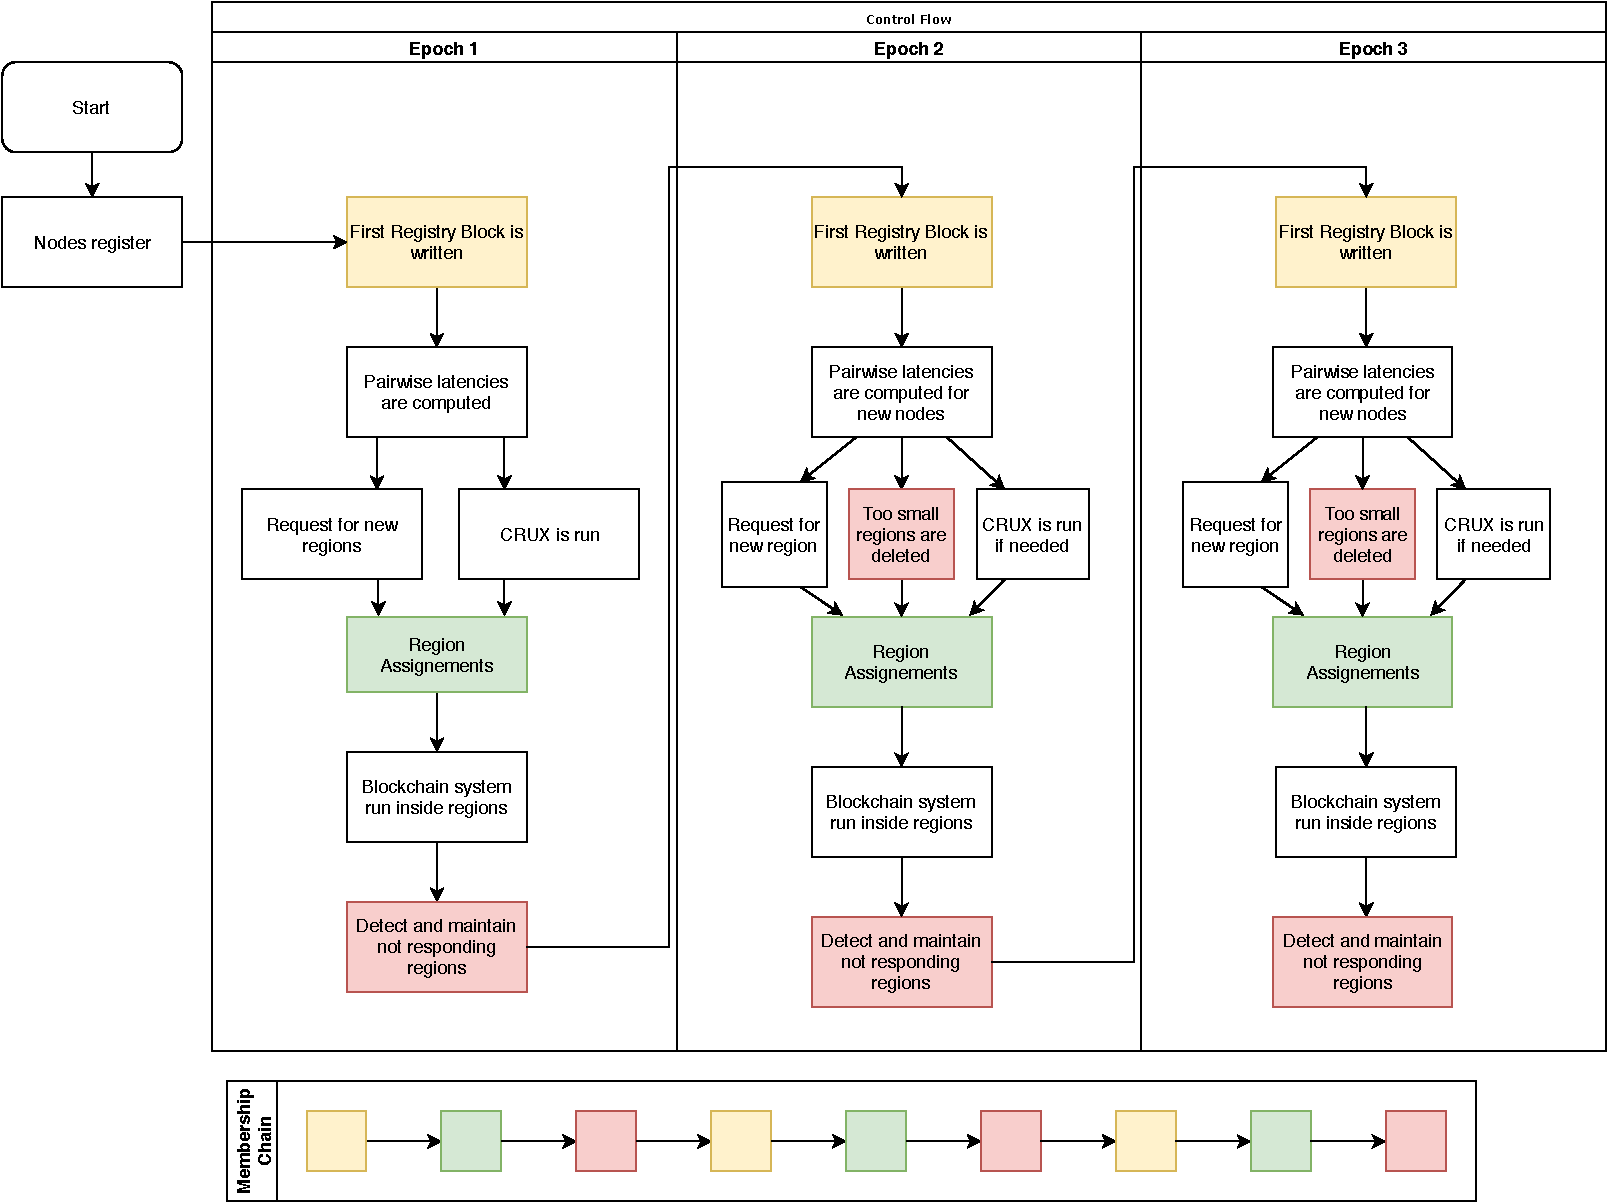
\includegraphics[width=400pt]{figures/Nyle_controlflow} \caption{General control Flow
of Nyle} \label{fig:controlflow} \end{figure}

\section{First version : Simple Control plane} This version presents the first
version of the Control Plane. In which most of the work is done on the
membership component. At each epoch nodes can join if they manage to get an
approval from the member of the previous region. The locality component in this
model is brute force : every node computes its pings to every other nodes and
consencus is made on that information. The region component in this model is
really simple : based on the registration, and the pings, CRUX is run at each
epoch. Redrawing the map of the entire system. 


\subsection{Membership Protocol}
This section describes the membership protocol [FIG. \ref{fig:registrationprotocol}].


\begin{figure}[!h] 
\centering
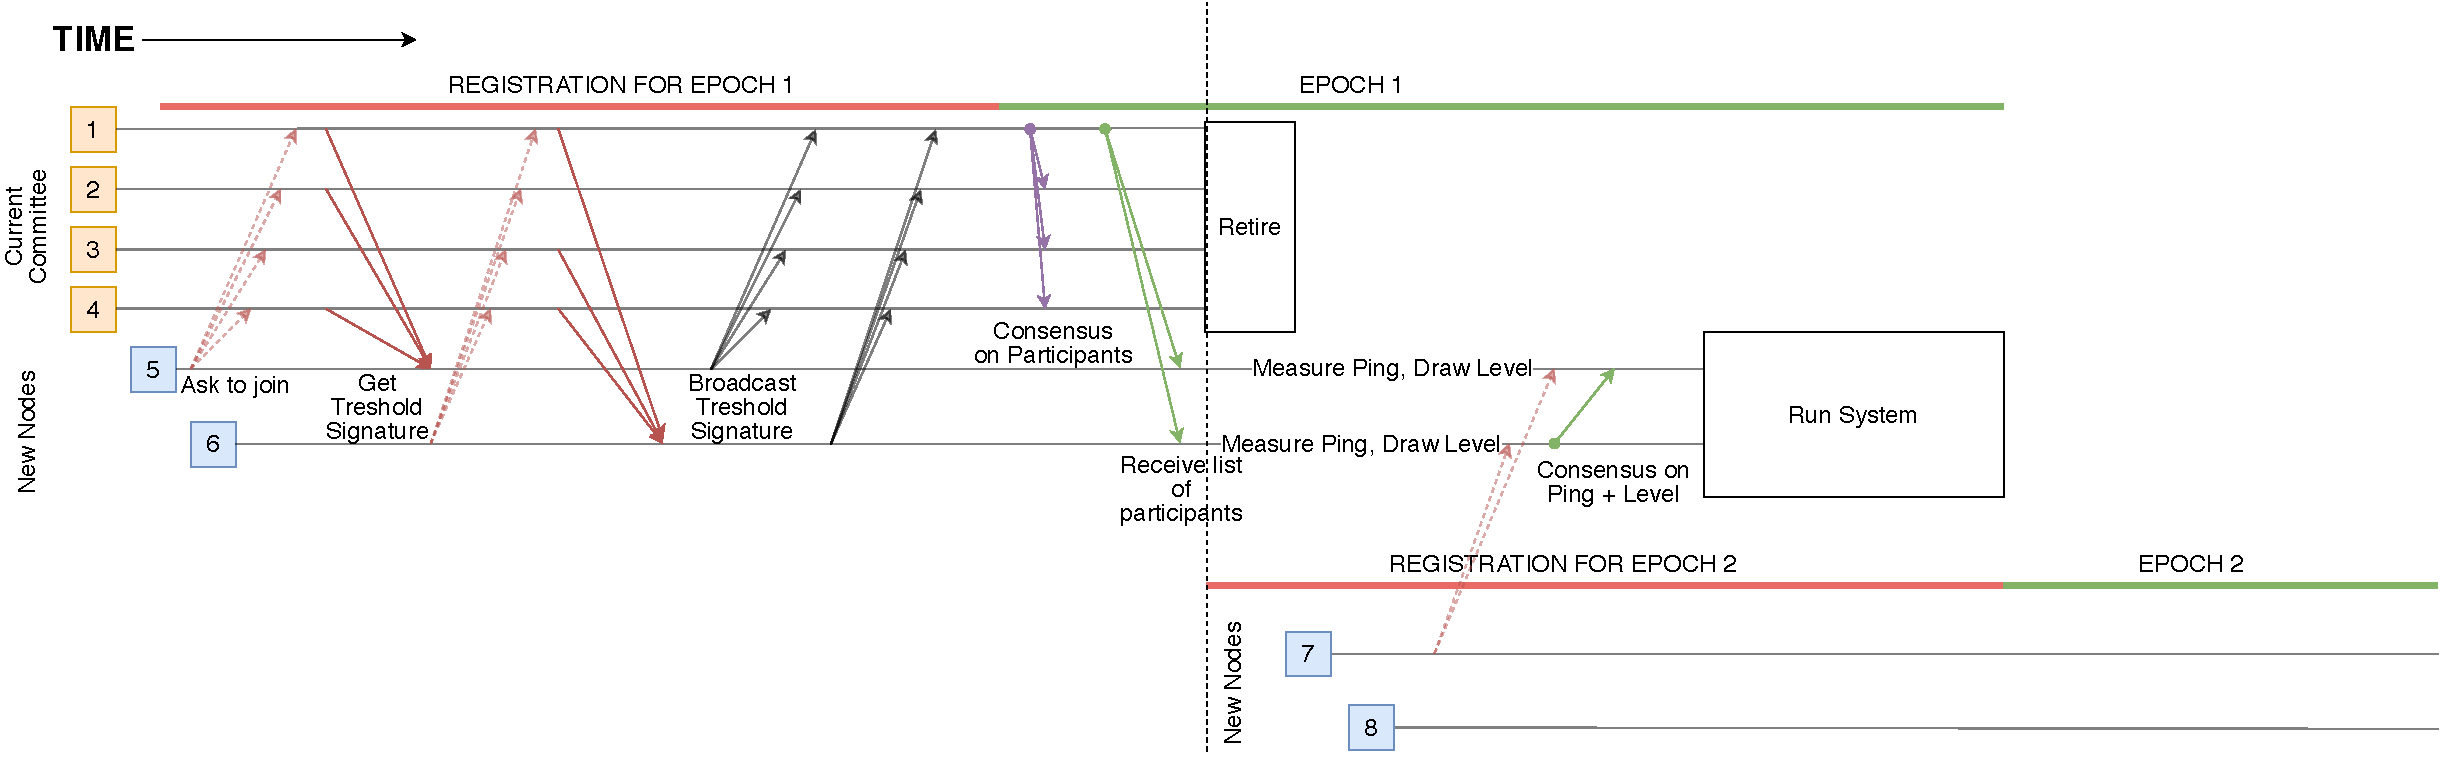
\includegraphics[width=400pt]{figures/Registrationprotocol}
\caption{Sketch of the protocol}
\label{fig:registrationprotocol}
\end{figure}

The system will go through some cycles (called epoch) of two different phases :
the registration period and the live period. The first period is actually there
to manage the participants of one current epoch, and the “underlying system”
(for example a cruxified-blockchain) will be run during the live period. Assume
that each node has a synchronized wall-clock which gives the time of the
different periods.

The authority that will decide which node participates in the next epochs are
the participants of the current epoch, which will be called the admission
committee. Assume that a set of genesis participants, which will be the first
admission committee, exists.

\paragraph{Registration Period}
If a node wants to register for the next epoch, it has to send the following
information to the admission committee : a name, a public key, and an
endorsement (for example solution to a proof-of-work problem) and ask for a
threshold-signature. 

If the new node manages to get back a threshold-signature from the current
committee, it has to broadcast it again to the admission committee during the
same registration period. The current committee will then acknowledge that it
is a participant for the next epoch. The admission committee will aggregate the
threshold-signatures for all the participants for the next epoch. At the end of
the registration period, the admission committee will reach a consensus on the
new participants, by threshold-signing the list of the members.  

\paragraph{Live Period}
At the beginning of the live period, one member of the admission committee will
send the threshold-signed list of the participants to the current members. If
one of the participants did not receive the list, it can ask any member of the
admission committee to have it. After that propagation, the admission committee
can retire, and the member of the current epoch becomes the new admission
committee. Then members of the new epoch will compute ping-distances between
each other. Participants will as well draw a level from unpredictable,
bias-resistant public randomness source. They will then reach consensus on
those ping-distances and levels by threshold-signing them and rebroadcast them.
At this point each member of the new epoch will have the same view of the
system (participants + pings + levels). Therefore these participants will be
capable of running the system in a deterministic manner.

Following the election of the new admission committee at the beginning of the
live-epoch, the registration period for the next epoch can begin, as the
authority that will accept admission is running. Registration period and live
period can therefore be superposed [FIG. \ref{fig:registrationprotocol}], which
permits to have a system running at every time. 

\subsection{Threshold-signing admission}
To get an admission a node that wants to join for the next system will use the
BlsCoSi protocol \cite{BlsCoSi_protocol}. it will generate a tree with him as
the root and the admission committee as nodes in the tree. Each node of the
admission committee will have the choice of signing or rejecting the admission
query. The threshold will be set at the majority. So if a node manages to get a
majority of signatures then it will be accepted in the system, A node from the
admission committee is supposed to accept the query if it has not already seen
the node, and if the endorsement is convincing and was made with the public-key
associated. This ensures that a node cannot steal the endorsement of another
for registration.  

%%%%%%% Committee consensus
\subsection{Committee consensus}
Committee consensus is used at two different times. First at the end of the
registration period. Consensus should be reached by the admission committee to
the participants of the next epochs. A random member of the admission committee
is selected to run the consensus protocol. It will send the list of members
that it aggregated during the registration period. And try to get a threshold
signature on it from the other member of the admission committee. Members of
the admission committee are supposed to sign the list if they aggregated the
same list of members for the next epoch.

If one member does not manage to reach consensus, another can be selected to
run the consensus. A communication round can be added between two consensus
phases in order that every member of the admission committee broadcast its list
of members with valid proofs.

The same idea is used at the beginning of the live epoch to reach consensus on
the list of pings between every member of the system and on the levels on all
nodes in the system.

% TODO : think on what to do if the consensus is not manageable. 

\section{Discussion}
\subsection{Advantages}
This simple version of the control plane is actually solving the problem of
churn and nodes movement in the system. A comparison will be made with a fixed
version only using CRUX for region management but without control plane. The
system begins with a fixed number of nodes and create regions based on CRUX,
then the system is replicated inside all regions. 

\subsubsection{Nodes insertion}
The version without control plane cannot add nodes to the system. Indeed a
fixed number of nodes is required to create the regions. With this control
plane, node insertion is possible at the beginning of every epoch.
% TODO add image


\subsubsection{Churn resistance}
Nodes can churn. If the system is not supposed to change, crashing nodes can be
still in the system. With this control plane, nodes that have crashed cannot
register for the next epoch and therefore are removed from the system. 
% TODO add image 


\subsubsection{Adaptation to node movements}
Nodes can move as well, if the regions are only drawn at the beginning of the
system. Then it's possible that after a while a lot of nodes have migrated from
where they were at the time that the regions were drawn. This might be a
problem, indeed, the purpose of the replication was to ensure that in case of a
partition, nodes participating in the same side of the partition should still
be able to work. If most of the nodes have moved, but are still participating
in the region of their first assignment, a partition could happen somewhere in
the system leading to failing regions that should be on the same side of the
partition. The control plane solves this problem as the region are redrawn at
each epoch taking account of the movement of the nodes. Increasing the
partition resistance, with the movement of nodes.
% TODO add image

\subsection{Drawbacks}
This control plane is simple and reach its objective, but it requires a lot of
resources. Some of the drawbacks of this approach are listed below. 
These drawbacks are addressed in the section Improvements.  

\subsubsection{Control Plane is global}
If the system is replicated in all the regions, the control plane itself is
global. Meaning it could be subject to a partition. In this case the replicated
system would continue to work, but the control plane could only continue to
work on the side of the majority. This is not a major drawback as the main
purpose, the continuity of the subordinate system is guaranteed.

\subsubsection{Epoch transition requires resources}
Epoch transition requires a lot of resources, indeed first it needs a lot
communication for the consensus and the registration as every nodes that were
previously on the system should be contacted by every new nodes. If $N_i$ is
the number of participants at epoch $i$. Then registration for epoch $i+1$
requires $O(N_i * N_{i+1})$ messages. As every new nodes have to send a message
to every member of the previous committee. This can be really inefficient. 

Then when the registration is done, the protocole as it is will redraw most of
the regions as the algorithm for region creation is reused. This can be
inefficient as well, and it then for the transition to happen, a copy of the
whole underlying system at epoch $i$ should be replicated in each new region of
epoch $i+1$.
 
\subsubsection{Omniscience of the nodes}
Nodes are actually aware of a lot of information. By design they are aware of
the list of every other nodes in the system, their levels, the pings between
each pair of nodes in the system, all the region created and all the region
assignment. The nodes needs to be aware of these information in order that
every nodes will run the algorithm for region creation and arrives to the same
regions. But this can be a lot of information to store.

\section{Security Analysis}


%%%%%%%%%%%%%%%%%%%%
\chapter{Improvements}
%%%%%%%%%%%%%%%%%%%%
This section proposes improvement to the simple control plane approach. They
are supposed to address drawbacks of this simple protocol, each improvement
will be illustrated in a Strawman model. At the end of Strawman, an advanced
version of the control plane that uses a region creation algorithm based on
time/space graphs will be proposed. 

\section{Strawman 1 : Locarno Treaties}

Following the First World War, it was decided that the borders of Germany
should remain fixed. The Locarno Treaties defined some of these borders. The
idea of this Strawman model in not to let the borders of regions change more
than defined. The rules for evolving from one epoch to another are defined. The
idea is to use a deterministic set of rules, based on the ping, the
registrations and the map of the previous epoch to draw the map of the current
epoch using the less redrawing as possible. CRUX is run at the first epoch
giving the first version of the system. Registration is still global and each
node will have all the information about the memberships of every node.Then
from one epoch to another, the purpose of the game is to keep as much region as
possible without breaking the locality rules.

\subsection{Rules for a node }
This section describes how to transform the regions from one epoch to another.
The point of view of one node that stays fixed in the system is taken, the goal
is that node can keep most of its region assignment.  What are the
implications. As it was said other nodes might join, leave or move. This leads
either to change in its cluster of in its bunch. 

\subsubsection{Nodes leaving the cluster} 
This will shrink the cluster. As the regions created by a given node stops when
the radius covers the whole cluster, this might lead to the deletion of some
regions, note that the smallest one is still kept. This does not change the
region assignment and the nodes can still keep the replicated system of the
previous epoch running.

\subsubsection{Nodes joining the cluster} 
On the contrary, if nodes join the cluster, this might lead to the creation of
additional region to cover these extra nodes. The node will then replicate its
system to the newly created regions. But most of the regions are kept the same.

\subsubsection{Nodes leaving the bunch} 
Nodes participate to all the region in their bunch, leading to participate to
the whole system. If a node left the system in the bunch,  this leads to a
region centered around a point that is not in the system anymore, but other
nodes participating in that region might still be in the system. A random node
participating in that region could be chosen to be responsible for the maintain
of that region.  Or this region assignment can be forgotten. 

\subsubsection{Nodes joining the bunch} 
If nodes are joining in a bunch, this leads to additional region assignment. 

\subsection{Rules for the levels.}


\textit{In the space-time graph (the image), most of the regions remain the same and
the modifications appear in small places.}

\section{Strawman 2 : Fog of the War}

Each node of the system will have a different view of the world at a given time
depending on its place in the system and its interactions. Again the idea is
that one node should be aware of only the information it needs to perform its
actions. 

A correspondence can be made with the fog of war in some traditional real-time
strategy video game. Where each player will have its own view of the system,
based on where it is now (real-time evolution), where it was in the past but
cannot see now (fog) and what it has not already seen (dark).

Each player view will evolve through space and time accordingly. In the context
of the game, the advantage of this view is that it hides the adversarial
strategy. In the context of our system, this view will hide most of the
information that is not relevant to one node but allow it to perform its
operation without the storage and/or communication overhead. 

The design of this Strawman will be the following. Each node declares a
position during the registration, and other nodes computes their bunch and
cluster according to this declared position. Each node will therefore be able
to compute their bunch and cluster based on these declared position. To ensure
the correctness of the system a random committee of checkers are elected after
the registration process. These checkers will perform some tests (pinging other
nodes of one region) and publish the results. 

\begin{figure}[!h] 
\centering
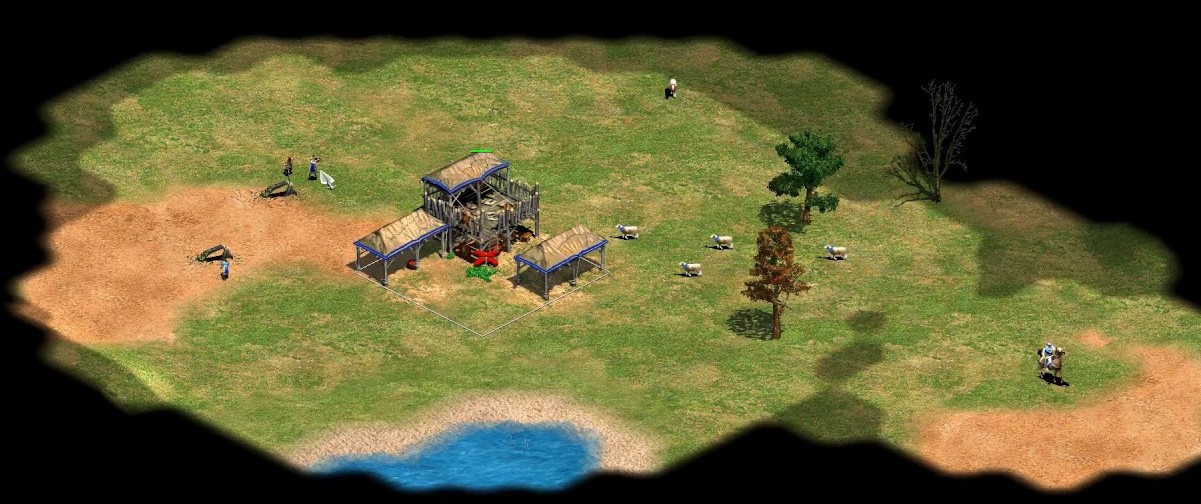
\includegraphics[width=400pt]{figures/fog_of_war}
\caption{Fog of war representation in a classic real-time strategy video game. }
\label{fig:registrationprotocol}
\end{figure}

\section{Introducing the Space/Time metrics}

Pings give a space/time insight of the evolution of the system.  This idea can
be leveraged to create the Space/Time version of the control plane.In fact
every message (send + reply - processing time) can be transformed to be used as
a ping as well. Therefore each time a node interacts with other nodes it can
use that additional information to get insight about the evolution of the
system. 

What type of information can be inferred from this additional method ? First
nodes can track the evolution through time and space of other nodes in the
system. And react to them. For example, if a new node manages to ping an
existing node from inside one region, the already existing nodes could trigger
registration of these nodes. On the contrary, if one node starts to get away
from the rest of the region, then other nodes will notice and can decide to
kick this node out of the system (after consensus with the existing nodes).
Modifications (e.g. nodes movement, churn), can be detected directly with the
messages, and the system can react to it. Churn can be interpreted as a node
movement in this model, with the churning node moving to infinity. If one
moving node is leaving one region, this information can be propagated to the
directly upper region containing the node. 

\subsection{Information as bubbles in space time graphs}

Imagine the following situation : there is a system of some nodes divided into
regions. All nodes are fixed except one which is moving. While moving this node
is interacting with other nodes (sending messages and executing query for the
system). Other nodes detect its movement, and are capable of reacting to it.
This movement triggers some action : joining regions and leaving others. If the
node is moving slowly, the reaction stays local, as information only needs to
be propagated in some upper region to be resolved. On the contrary, if the node
moves fast, then it generates bigger bubbles, it goes to the biggest region to
be resolved.  Structurally this view of the system is not really different from
the one that we described before, but philosophically this view goes much
deeper as it taking in account the interactions of the nodes in a space/time
matter.

Recall that nodes participate to all region that is bigger than its cluster. If
nodes in one region detect that another is moving apart, they do not expect it
to participate in this region anymore and they propagate the information in the
directly upper region. This is done recursively till the node is again included
in the more global region.  In the opposite, if a region detect that one node
is approaching it expects it to participate in the region, and propagate the
information in the directly upper region.

If a node churns, then this information is propagated all the way to the
biggest region, and the node is excluded from the system.  If a node joins the
system, it starts to ping some nodes for information. It can ask for the list
of participants and pings everybody. When it starts pinging some nodes that are
close to it, these nodes detect that a new node wants to join the system and
expect it to enter the system.  



%%%%%%%%%%%%%%%%%%%%
\chapter{Conclusion}
%%%%%%%%%%%%%%%%%%%%

In the conclusion you repeat the main result and finalize the discussion of
your project. Mention the core results and why as well as how your system
advances the status quo.

\cleardoublepage \phantomsection \addcontentsline{toc}{chapter}{Bibliography}
\printbibliography

% Appendices are optional \appendix %%%%%%%%%%%%%%%%%%%%%%%%%%%%%%%%%%%%%%
% \chapter{How to make a transmogrifier} %%%%%%%%%%%%%%%%%%%%%%%%%%%%%%%%%%%%%%
%
% In case you ever need an (optional) appendix.
%
% You need the following items: \begin{itemize} \item A box \item Crayons \item
% A self-aware 5-year old \end{itemize}

\end{document}
